\section{Camera configurations}
\label{app:views}
Table~\ref{tab:configs} lists the camera configurations in the processed set: the view string from the camera metadata, the sensor column offset of the region of interest, the number of discharges, the spread of $R_{\rm LCFS}$ across the discharges, the Spearman correlation between limb-peak column and $R_{\rm LCFS}$, the configuration's own scale where it could be fitted, and whether the configuration uses its own scale or the pooled campaign scale (Section~\ref{sec:calibration}).

\begin{table}[h]
\centering
\scriptsize
\setlength{\tabcolsep}{4pt}\begin{tabular}{llrrrlll}
\toprule
Camp. & View string & ROI left & Shots & $\Delta R_{\rm LCFS}$ (cm) & $\rho$ & Scale (mm/px) & Used \\
\midrule
M6 & HM10, normal, f/1.8 & 193 & 70 & 13 & -0.94 & 2.9 (2.7--3.0) & own \\
M6 & HM10, normal & 193 & 61 & 17 & -0.89 & 3.7 (3.1--4.1) & own \\
M6 & hm10 midplane f4 & 193 & 59 & 22 & -0.47 & 3.9 (3.6--5.1) & pooled \\
M6 & HM10, normal, D$\alpha$ 10 nm & 193 & 30 & 7 & -0.88 & 3.5 (3.2--3.9) & own \\
M6 & HM10, normal & 257 & 14 & 10 & +0.34 & 0.9 (0.4--1.9) & pooled \\
M6 & HM10, normal, D$\alpha$ 10 nm & 513 & 7 & 6 & -- & -- & pooled \\
M6 & hm10 midplane f4 & 161 & 6 & 4 & -- & -- & pooled \\
M6 & HM10 - upside down & 193 & 3 & 1 & -- & -- & pooled \\
M6 & probe 100kHz & 193 & 3 & 6 & -- & -- & pooled \\
M6 & HM10, normal, D$\alpha$ 10 nm & 545 & 2 & 0 & -- & -- & pooled \\
M6 & HM10, normal, D$\alpha$ 10 nm & 225 & 1 & 0 & -- & -- & pooled \\
M6 & HM10, normal & 225 & 1 & 0 & -- & -- & pooled \\
M6 & probe view & 193 & 1 & 0 & -- & -- & pooled \\
M7 & HM10 & 193 & 22 & 13 & -0.88 & 3.3 (3.0--3.8) & own \\
M7 & HM10 & 257 & 3 & 1 & -- & -- & pooled \\
M8 & HM10 f/2.8 4.8mm nd 0.9 & 193 & 32 & 21 & -0.58 & 5.2 (3.6--11.5) & own \\
M9 & HM10 + D$\alpha$ filter & 193 & 38 & 29 & -0.82 & 2.7 (2.5--3.4) & own \\
M9 & HM10 & 193 & 6 & 4 & -- & -- & pooled \\
M9 & HM10 f/2.8 4.8mm & 129 & 4 & 9 & -- & -- & pooled \\
M9 & HM10 + D$\alpha$ filter & 129 & 1 & 0 & -- & -- & pooled \\
M9 & HM10 + D$\alpha$ filter & 513 & 1 & 0 & -- & -- & pooled \\
M9 & HM10 + D$\alpha$ filter & 577 & 1 & 0 & -- & -- & pooled \\
M9 & HM10 & 129 & 1 & 0 & -- & -- & pooled \\
\bottomrule
\end{tabular}

\caption{Camera configurations and their calibration. A configuration uses its own scale when it has at least 8 discharges, at least 3~cm of spread in $R_{\rm LCFS}$, a correlation of the right sign with $|\rho| \ge 0.5$, and a bootstrap interval that excludes zero.}
\label{tab:configs}
\end{table}

\section{Within-shot calibration}
\label{app:calibration}
A within-shot regression of the limb-peak column on $R_{\rm LCFS}$ uses the few centimetres of plasma movement during a flat top. For the \nWithinShot{} discharges in which the LCFS moves by at least 2~cm, the implied scale has a median of \withinScaleMed{}~mm per pixel with an interquartile range of \withinScaleQLo--\withinScaleQHi{} and extremes below 1 and above $10^{\withinScaleMaxLog}$. The spread comes from three effects: the EFIT boundary is least reliable at the start and end of the flat top, where most of the movement occurs; the brightness profile changes shape as the density rises, which moves the peak at fixed $R_{\rm LCFS}$; and the lever arm is short, so a 1~cm error in $R_{\rm LCFS}$ changes the slope by tens of percent. The between-shot regression of Section~\ref{sec:calibration} replaces a few centimetres of movement in one discharge with 10--20~cm of position variation across a campaign and is correspondingly more stable.

\section{ELM detection}
\label{app:elm}
Figure~\ref{fig:elm} shows the $D_\alpha$ trace and the camera frame-mean brightness for an ELMy discharge, with the detected spikes. The camera proxy finds the same events as the $D_\alpha$ monitor where both are available and serves as the only detector where the $D_\alpha$ channel is missing.

\begin{figure}[h]
\centering
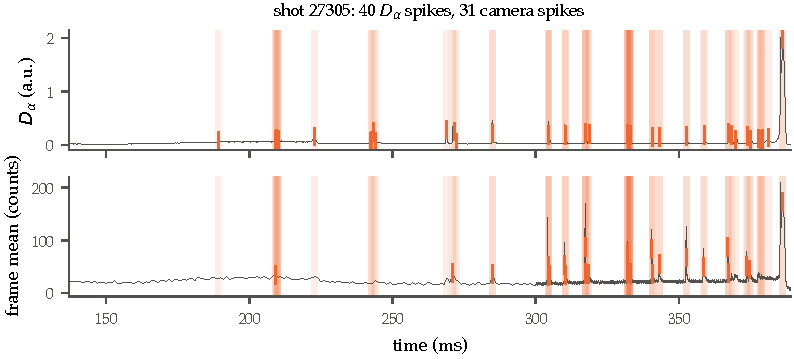
\includegraphics[width=\linewidth]{figs/fig_elm.pdf}
\caption{ELM detection on an ELMy discharge. Top: midplane $D_\alpha$ with detected spikes marked. Bottom: camera frame-mean brightness with its own spike detection. The shaded bands are the $\pm 1$~ms exclusion windows.}
\label{fig:elm}
\end{figure}
